% put here just enough to compile it 
\documentclass{article}
\usepackage{xcolor}
\usepackage[english]{babel}
\usepackage{graphicx}
% \usepackage{docincludes}
\usepackage{siunitx}

\usepackage{hyperref}
\usepackage{cite}
\usepackage{amssymb}
\usepackage{amsmath}
\usepackage{todonotes} % use \todo{WP2Leader: xyz} \todo{ESRz: xyz} or \todo[inline]{} for simple notes.
\usepackage{docincludes} %Added
\usepackage{mathtools} %Added for \prescript
\usepackage{algpseudocode}
\usepackage{algorithm}

\definecolor{deepblack}{rgb}{0,0,0}
\definecolor{deepblue}{rgb}{0,0,0.8}
\definecolor{deepred}{rgb}{0.6,0,0.4}
\definecolor{warningRed}{rgb}{1,0.2,0.2}
\definecolor{deepgreen}{rgb}{0,0.65,0}
\definecolor{commentgreen}{rgb}{0.5,0.7,0.5}






% is the format okay? format?? 
\usepackage[a4paper,top=2cm,bottom=2cm,left=3cm,right=3cm,marginparwidth=1.75cm]{geometry}
\title{Odin Multibody Dynamics Code}

\begin{document}
\begin{titlepage}
\maketitle
\thispagestyle{empty}

\begin{center}
{\includegraphics*[height=3cm]{figures/thread-logo}}
\end{center}

\begin{center}

\includegraphics[scale=0.3]{figures/flag_yellow}
\end{center}
\vspace*{1.3cm}
\begin{center}
\large{\sffamily{This project has received funding from the European Union's Horizon 2020 research and}}\\
\large{\sffamily{innovation programme under the Marie Sk{\l}odowska-Curie grant agreement No 860124.}}
\end{center}

\end{titlepage}
\tableofcontents
\newpage
%\input{methods.tex}
\section{Test cases with ODIN}\label{sec:testcasesodin}
\subsection{Introduction}

The preforms for resin impregnation in composites are typically manufactured by the deposition of a high number of slender textile yarns on the surface of a rigid body with complex geometry (mandrel). For the modelling of the yarn-to-mandrel contact interactions, the mandrel can either be modelled as a rigid body or as a beam for the specific case of a cylindrical geometry of the mandrel. In the following numerical tests, both cases have been studied. In the first test, a cylindrically shaped mandrel is modelled as a stocky and fixed beam, along with two slender textile yarns in contact with the mandrel. Further in the second test, the mandrel is modelled as a rigid body with contact-friction interactions modelled as beam-to-rigid body contact.

\subsection{Mortar contact for yarn-mandrel interactions}
\subsubsection{Test case description}
%same text as just before
%The preforms for resin impregnation in composites are typically manufactured by the deposition of a high number of slender textile yarns on the surface of a rigid body with complex geometry (mandrel). For the modelling of the yarn-to-mandrel contact interactions, the mandrel can either be modelled as a rigid body or as a beam for the specific case of a cylindrical geometry of the mandrel. 
In this numerical test, a cylindrically shaped mandrel is modelled as a stocky and fixed beam, along with two slender textile yarns in contact with the mandrel.\\
The textile yarns are modelled as geometrically exact beams using the Lie group $SE(3)$ formalism presented in \cite{sonneville2014geometrically}. On deposition on the mandrel surface, the contact forces are modelled either as concentrated point forces (for large contact angles) or distributed over a continuous patch (for acute contact angles). The mandrel is modelled as the master beam and the yarns as the slave beams. A Lagrange multiplier shall be used to denote the contact pressure, which is discretized using standard linear shape functions for first-order interpolation. For the quasi-static case, the discrete equilibrium system is formulated and presented in \cite{bosten2022mortar}:
%
\bea\label{equilibrium}
\boldsymbol{\mathrm{f}}^{\textrm{int}}(q) + \boldsymbol{\mathrm{B}}^{T}(q) \boldsymbol{\lambda} &=& \boldsymbol{\mathrm{f}}^{\textrm{ext}}(q)\\ %\label{quasistatic}
\boldsymbol{\mathrm{0}} \leq \boldsymbol{\lambda} \perp \boldsymbol{\mathrm{g}}^{\textrm{con}} &\geq& \boldsymbol{\mathrm{0}} \label{LCP}
\eea
%
Equation (\ref{LCP}) represents a linear complementarity problem (LCP) which is further solved using an augmented Lagrangian formulation. 
The quantities $\boldsymbol{\mathrm{f}}^{\textrm{int}}$ and $\boldsymbol{\mathrm{f}}^{\textrm{ext}}$ are internal and external force vectors respectively, $\boldsymbol{\mathrm{B}}$ is the constraint gradient, $\boldsymbol{\lambda}$ are the Lagrange multipliers and $q$ is the configuration variable, and $\boldsymbol{\mathrm{g}}^{\textrm{con}}$ is the weighted normal constraints. For element $e$, it is defined as: 

\begin{equation}
    \boldsymbol{\mathrm{g}}_e^{\textrm{con}}(q_e) = \int_{s^e_{a}}^{s^e_{b}} \boldsymbol{\mathrm{N}}^{T} g \, \mathrm{d}s_1
\end{equation}
which is defined on the slave beam ($s_1$) along with shape functions $\boldsymbol{\mathrm{N}}$ defined as $\boldsymbol{\mathrm{N}} (s_1) = \begin{bmatrix}
\frac{s_1}{L_{e_1}} & 1 - \frac{s_1}{L_{e_1}} 
\end{bmatrix}$. 

\subsubsection{Simulation setup}
A quasi-static frictionless simulation of two beams deposited on the surface of a stocky and fixed beam is performed using Odin multibody dynamics research code \cite{odin2022}. The radius of the slender beam is $r_y = 0.002$ m along with the length $l_y = 5$ m. Similarly, the radius of the stocky beam is $r_m = 0.2\,$m along with length $l_m = 5\,$m. The yarns and mandrel are discretized using 40 beam finite elements and the material properties of basalt fibres are assigned for the yarns as $E = 90\,$GPa, $\nu = 0.21$ and $\rho = 2750\,$kg/m$^3$ and properties of steel assigned to the mandrel i.e. $E = 200\,$GPa, $\nu = 0.3$ and $\rho = 7750\,$kg/m$^3$. A spherical joint is used at the starting positions of the slender beams to allow rotation. On the contrary, the stocky beam is fully constrained using a clamped boundary condition.

\subsubsection{Results}
The cross-winding of two yarns on the mandrel surface is shown in Figure \ref{testsetup}. For performing the test, an MKL Pardiso linear solver (CSR matrix storage) has been used along with a Newton nonlinear solver for which the maximum iterations is set to 100 and a relative tolerance of $1\mathrm{e}{-4}$ as presented in the configuration JSON file. The simulation is performed for a total time $T = 12$ s with a time step size $h = 0.001$ s. The results are stored in an HDF5 file created, which is further used for post-processing together with Blender for visualization purposes.

\begin{figure}[h]
    \centering
    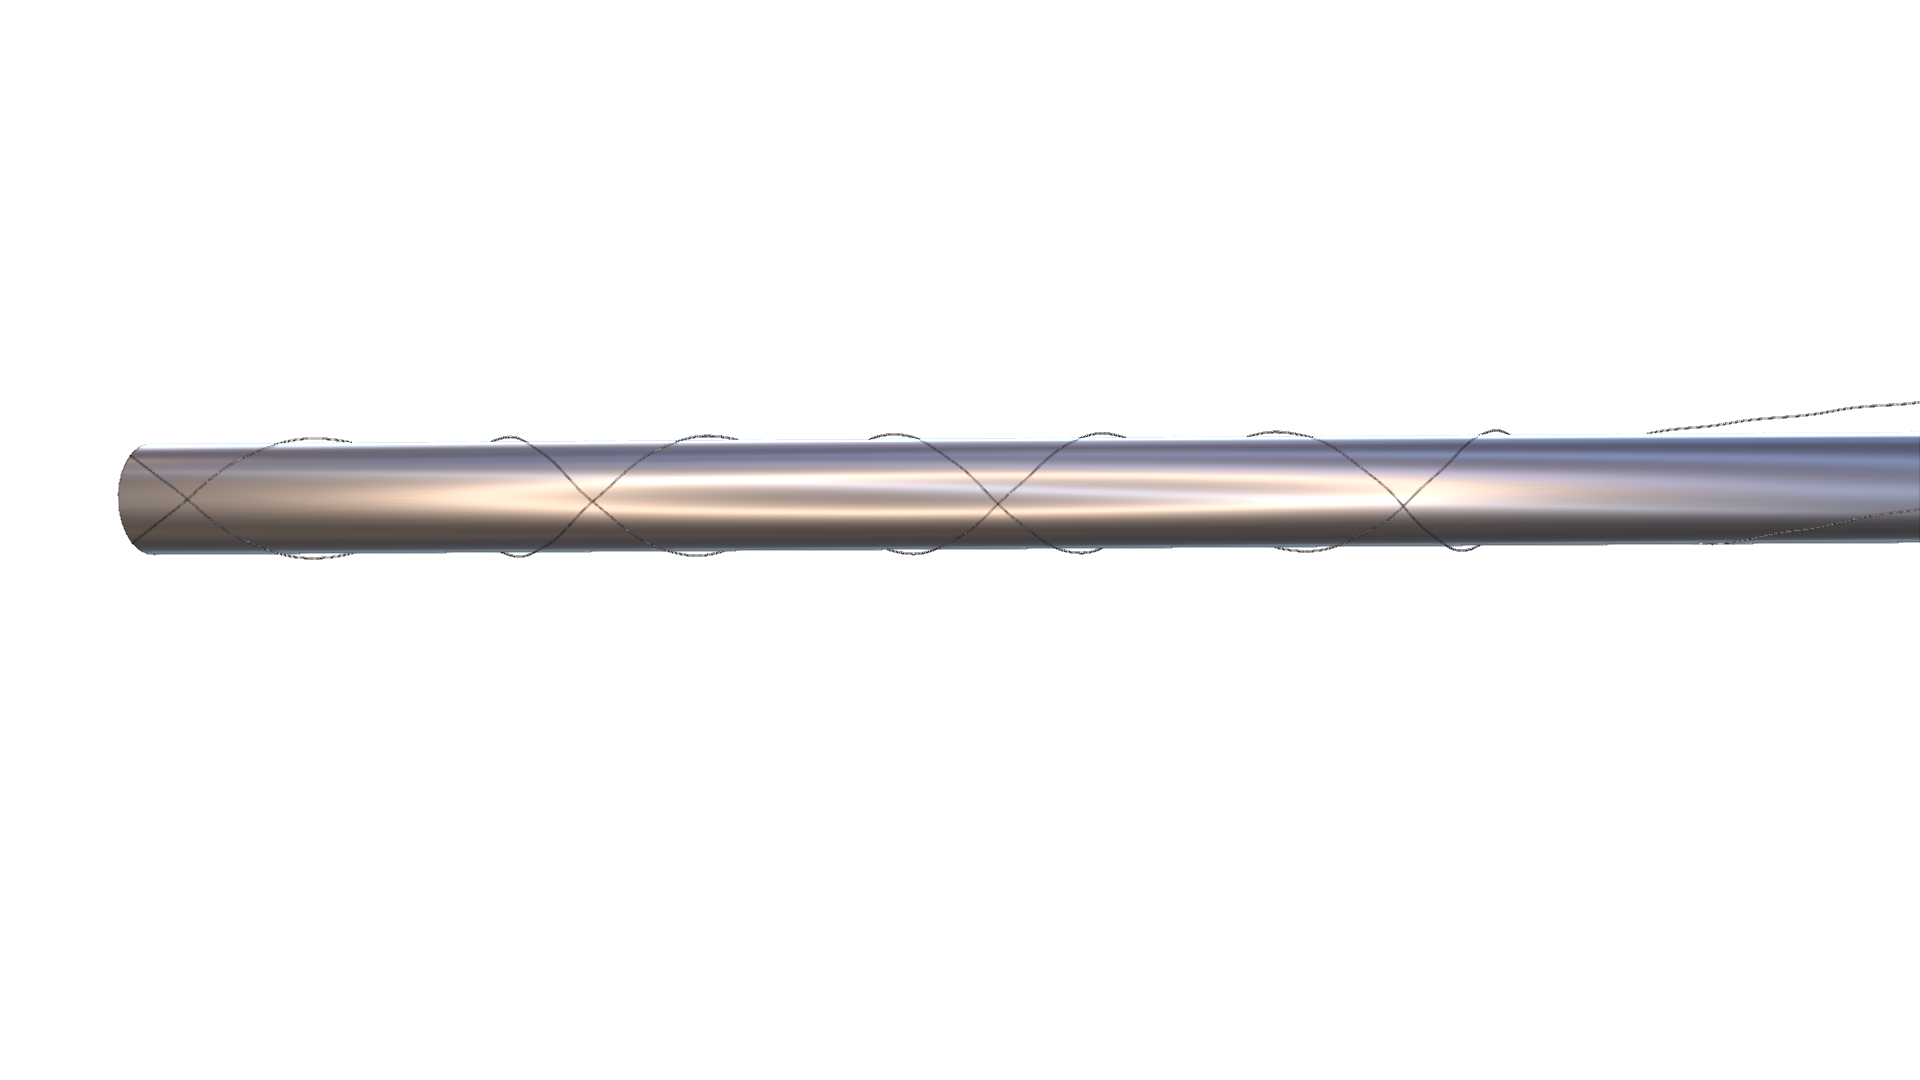
\includegraphics[width=400pt]{figures/mortaryarnmandrel_1.png}
    \caption{Yarn-to-mandrel frictionless interactions modelled using mortar formulation for line contact (mandrel modelled as a stocky beam).}
    \label{testsetup}
\end{figure}


















\subsection{Description of code: mortar contact for yarn-mandrel interactions}
Odin multibody dynamics research code \cite{odin2022} is written in C++ programming language. The philosophy of Odin relies on the use of nonlinear finite elements to represent the components of a multibody system. This is further accompanied by kinematic or contact constraints. The equations of motion are automatically assembled in Odin based on the specified choice of the mechanical analysis and further solved using the specified numerical scheme.\\

\subsubsection{Python code file} 
\begin{enumerate}
    \item The necessary modules are imported and Odin is initialized using \pythoninline{initialize_odin()}.
    \item A physical system is created which is the master container for all the components of the system, using \pythoninline{ps = create_physical_system()}. Additionally, the mechanical analysis and nodal frames are defined in the physical system. As a nodal frame is defined by translations and rotations, a \pythoninline{Vec3} (vector of 3 components) can be used for defining translations along with quaternions for rotations.
    \item The \pythoninline{JSON} file which configures the methods to be used (nonlinear solvers etc.) is loaded using \pythoninline{json_file = json.load(open())}.
    \item For defining the circular motion as the boundary condition for yarns, the radius \pythoninline{r_trajectory} is defined along with defining the radius of yarns \pythoninline{r}, length \pythoninline{l_beam} and mandrel dimensions. The number of finite elements to be used are defined as \pythoninline{nele_AB} and \pythoninline{nele_BC} for the yarns and mandrel beam respectively.
    \item The element and node labels are initialized as \pythoninline{elabel = 0} and \pythoninline{nlabel = 0}.
    \item For \pythoninline{nlabel = 0}, a grounded spherical joint has been defined by simply specifying the position of the joint and using the C++ element \pythoninline{Ground_SphericalJ} as :
    \pythonstyle
    \begin{tcolorbox}\begin{lstlisting}
    prop_spherical = SphericalJProps()
    prop_spherical.position = np.array(start_point_AB)
    ps.create_element("Ground_SphericalJ", elabel, [nlabel],
                        prop_spherical)
    elabel += 1 
    \end{lstlisting}\end{tcolorbox}
        The elabel has now been incremented using \pythoninline{elabel += 1}. In this way, no massless node is defined.
    \item The material properties and sectional stiffness coefficients of the beam are defined using the variable \pythoninline{params_beam}. 
    \item Using \pythoninline{beamAB_props}, the choice of using a tangent operator and geometric stiffness is defined with \pythoninline{True} or \pythoninline{False} as \pythoninline{beamAB_props.with_tg_operator = False}.
    \item The normal and binormal vectors of the orthonormal triad are defined as \pythoninline{n_0 = np.array([0, 1, 0])} ($Y$-axis) and \pythoninline{b_0 = np.array([0, 0, 1])} ($Z$-axis). Finally the beam is created in the physical system using:
    \pythonstyle
    \begin{tcolorbox}\begin{lstlisting}
    prepro.straight_beam(start_point_AB, end_point_AB, nele_AB, 
    elabel, nlabel, n_0, b_0, beamAB_props, ps)
    elabel += nele_AB 
    nlabel += nele_AB 
    n_beamAB_1 = nlabel
    \end{lstlisting}\end{tcolorbox}
        The \pythoninline{elabel} and \pythoninline{nlabel} are further incremented using \pythoninline{nele_AB} and \pythoninline{n_beamAB_1} is specified to label the last node of beam AB (yarn 1).
    \item Essential boundary conditions for circular motion are now defined using piecewise linear functions \pythoninline{PWLFunction()}. The prescribed circular motion is in the $YZ$ plane and therefore the remaining $4$ DoF are clamped. Also, the motion needs to be prescribed at position, velocity and acceleration levels as:
    \pythonstyle
    \begin{tcolorbox}\begin{lstlisting}
    bcx = BCValue(bcx_func, bcx_v_func, bcx_a_func)
    bcy = BCValue(bcy_func, bcy_v_func, bcy_a_func)
    bc.insert(n_beamAB_1, BC.Motion, [bc_clamp, bcx, bcy, bc_clamp, 
                                      bc_clamp, bc_clamp])
    \end{lstlisting}\end{tcolorbox}
    \item The similar structure is followed to define the mandrel as a stocky beam, but with fixed nodes (all $6$ DoF clamped) as:
    \pythonstyle
    \begin{tcolorbox}\begin{lstlisting}
    bc.insert(start_b2, BC.Motion, [bc_clamp, bc_clamp, bc_clamp, 
                                    bc_clamp, bc_clamp, bc_clamp])
    bc.insert(n_beamAB_2, BC.Motion, [bc_clamp, bc_clamp, bc_clamp, 
                                      bc_clamp, bc_clamp, bc_clamp])
    \end{lstlisting}\end{tcolorbox}
    \item The second yarn is defined in the similar structure as \pythoninline{beamAB}, but the circular motion is now in the opposite direction.
    \item Finally, the scaling and penalty parameters for the augmented Lagrangian are defined and the contact pairs are defined according to the convention that the first beam element passed to the contact element is the slave beam. Therefore, the yarn is defined as the slave and the mandrel as the master. Firstly, the contact pairs between the first yarn \pythoninline{nele_AB} and mandrel \pythoninline{nele_BC} are defined as:
    \pythonstyle
    \begin{tcolorbox}\begin{lstlisting}
    for i in range(nele_AB):
        for j in range(nele_BC):
            ps.create_element("Beam_Contact", elabel,
                              [i, i + 1, j + nele_AB + 1, j +
                              nele_BC + 2], contact_prop)
            elabel += 1
    \end{lstlisting}\end{tcolorbox}
    \item In a similar manner, the contact pairs are further defined between the mandrel and second yarn, with mandrel defined as master and the yarn as slave.
    \item The specified choice of the analysis scheme (\pythoninline{NonSmoothMortarStatic} is further defined and the mechanical analysis computes the solution using the \pythoninline{JSON} file.
    \pythonstyle
    \begin{tcolorbox}\begin{lstlisting}
    analysis.set_analysis_type(AnalysisType.NonSmoothMortarStatic)
    analysis.compute_solution(json_file)
    \end{lstlisting}\end{tcolorbox}    
\end{enumerate}

\subsubsection{JSON file}
In the \pythoninline{JSON} files, each of the components have at least two fields: \pythoninline{scheme} or \pythoninline{name} and \pythoninline{parameters}. The field \pythoninline{scheme} is used to identify numerical schemes and name is used to identify a component that is not a numerical scheme. The \pythoninline{field} parameter is used to specify any parameter needed to configure the specific scheme or name identifying the component to be created. You can observe that as scheme the \pythoninline{Newton_NL_Solver} is provided, which identifies as the Newton Nonlinear solver. As parameters, you have some properties which correspond to the nonlinear solver but also a \pythoninline{linear_solver} that in this case is set to \pythoninline{CSR_Pardiso_Solver}. This means that the direct intel MKL Pardiso solver is going to be used, assuming that the matrices are provided in CSR (Compressed Sparse Row) format. In addition, a component \pythoninline{Viewer} is defined and identified to name: \pythoninline{HDF5_Viewer}.

\subsection{Installation and running}
A Linux environment is preferred for Odin, although it can be used with a WSL ubuntu (or any virtual environment i.e. Oracle VirtualBox) on Windows. Additionally, \pythoninline{Visual Studio Code} is encouraged as the development environment, although any python notebooks (Jupyter Notebooks etc.) can be used. Odin has the option to automatically fetch and build the necessary third party libraries. Therefore, no additional installation procedures are needed. For the installation of Odin, please refer to the code documentation: \url{https://obruls.gitlabpages.uliege.be/doc4odin/firstSteps/index.html}.\\

Once Odin has been successfully installed along with the open source graphical software \pythoninline{Blender} for rendering, the python script example file can be run. It is important to note the \pythoninline{python} version being used to run the file, as it should be compatible with the \pythoninline{blender} version for rendering the simulation. The post-processing file reads an \pythoninline{hdf5} file format which is generated from the simulation. This \pythoninline{.h5} file is further imported into a python script written in \pythoninline{Blender} for the visualization of the simulation using \pythoninline{Pyblender}. 
\subsection{Beam-to-rigid body contact for yarn-mandrel contact-friction interactions}
\subsubsection{Test case description}
Following the numerical test on mortar line contact for yarn-to-mandrel interactions, the dynamic simulation shall now be studied. A beam-to-rigid body contact formulation with friction based on a collocation approach has been implemented to study the dynamics of yarn deposition on a mandrel surface. The neutral axis of the beam is represented by proxy discrete spherical collision geometries \cite{tasora2020geometrically} (of radius $r_s$ = radius of the beam). The mandrel surface is treated as the master plane and the collision elements as the slave. For the robust handling of a large number of frictional impacts, Newton-type solvers may suffer from ill-conditioning and singularity issues in the Jacobian. Therefore, a Gau{\ss}-Seidel solver is exploited which is well-suited for such problems.\\

The time discrete equations are solved using the decoupled version of the nonsmooth generalized-$\alpha$ time integration scheme \cite{cosimo2020robust} with the Gau{\ss}-Seidel solver So-bogus \cite{daviet2011hybrid}. Three decoupled sub-problems are solved using the splitting strategy as $\Delta \vectorbold{q}_{n+1} = \Delta \vectorbold{\Tilde{q}}_{n+1} + \vectorbold{U}_{n+1}$ and $\vectorbold{v}_{n+1} = \vectorbold{\Tilde{v}}_{n+1} + \vectorbold{W}_{n+1}$, where, $\Delta \vectorbold{\Tilde{q}}_{n+1}$ and $\vectorbold{\Tilde{v}}_{n+1}$ are smooth displacements and velocities, and $\vectorbold{U}_{n+1}$ and $\vectorbold{W}_{n+1}$ are position corrections and velocity jumps. 

\subsubsection{Simulation setup}
The transient simulation of the contact-friction interactions between a slender beam winding around a cylindrical rigid body is performed using Odin multibody dynamics research code \cite{odin2022}. The beam of radius $r_y = 0.001$ m and with length $l_y = 4$ m and material properties $(E = 90$ GPa, $\nu = 0.27$ and $\rho = 2670)$ Kg/m$^3$ has been used for winding around a cylindrical rigid body of radius  $r_m = 0.4$ m and length $l_m = 4$ m. The beam is discretized using 50 finite elements and spherical collision elements are attached to the nodes of the beam. A stiffness proportional Rayleigh damping has been used for structural damping. \\
 

\subsubsection{Results}
The investigation of the yarn-mandrel interactions has been performed in Figure \ref{fig:fricvalues} for one frictionless and two frictional cases ($\mu = 0.1$ and $0.4$). The time evolution of position of the center node of the beam (node 25) has been selected for the study. As expected in winding using a higher value of the friction coefficient ($\mu = 0.4)$, the sliding motion of the node is significantly postponed as compared to $\mu = 0.1$ and $0.0$. The simulation is performed for a total time $T = 8$ seconds with a time step size of $h = 0.005$.

\begin{figure}[h]
\centering
  \centering
  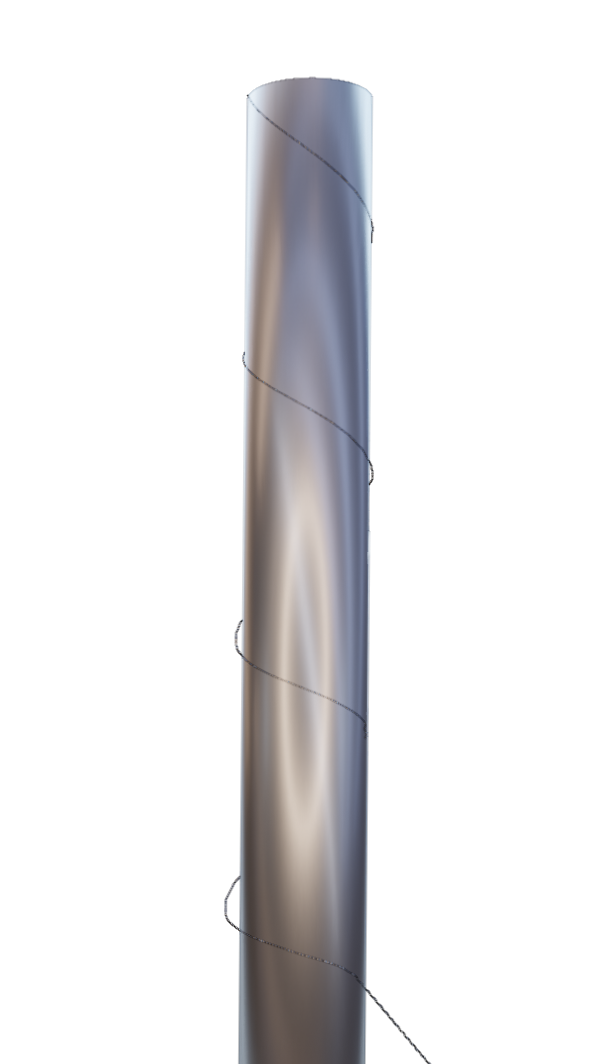
\includegraphics[width=0.27\linewidth]{figures/steel_mandrel_1.png}\\
  \centering
  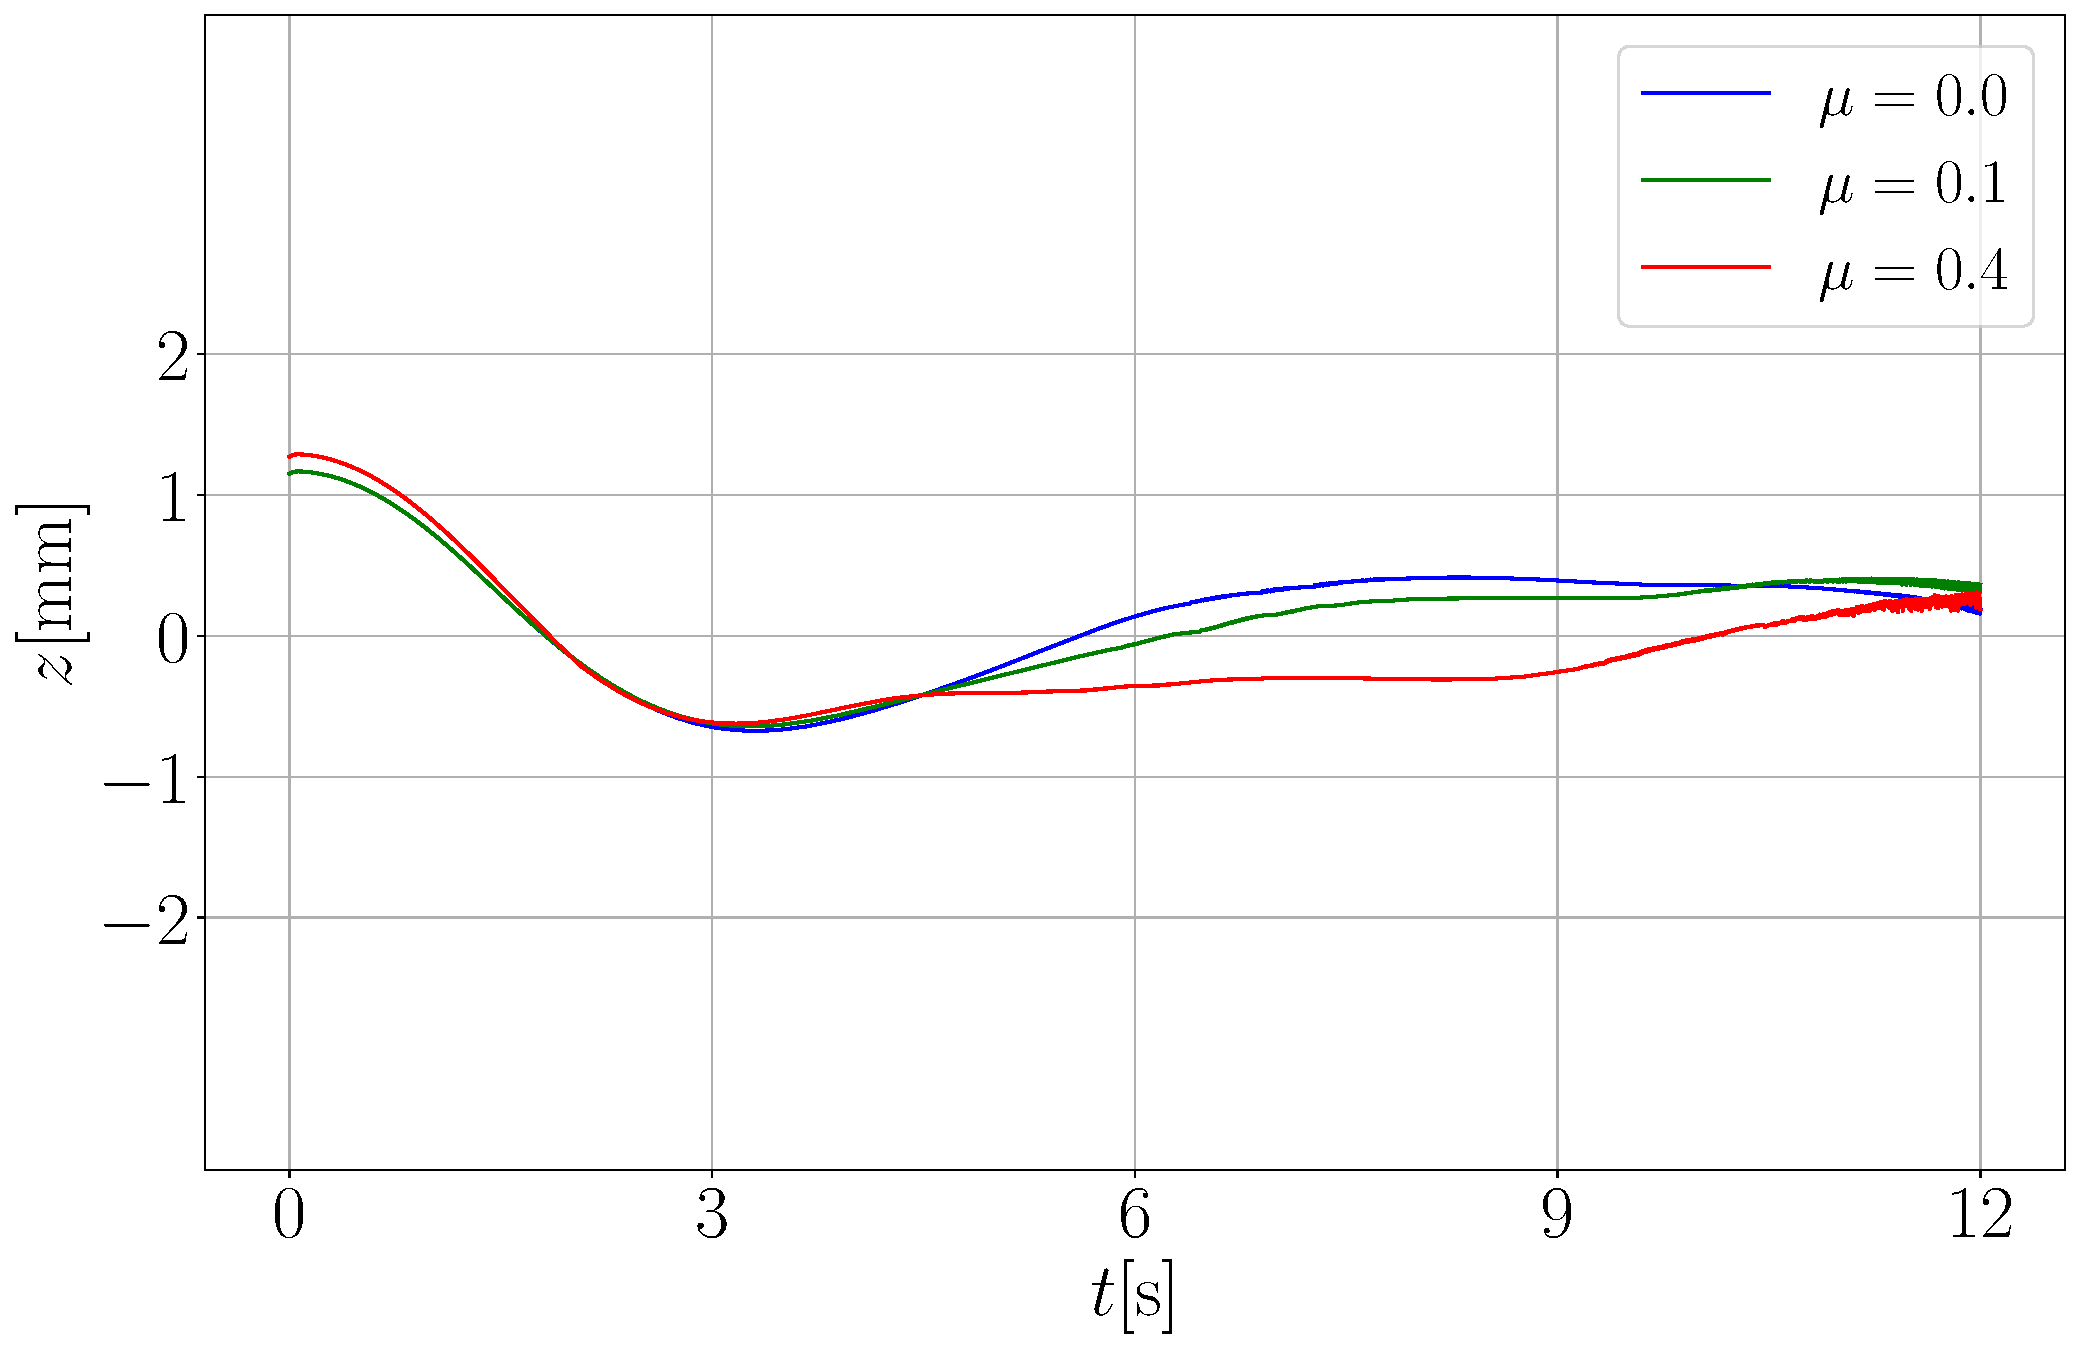
\includegraphics[width=0.47\linewidth]{figures/mu_compare.pdf}
\caption{Frictional dynamic yarn-to-mandrel interactions using beam-to-rigid body contact with a collocation approach. Time evolution of position of the center node of the yarn along the longitudinal axis (z) of the mandrel for different friction coefficients.}
\label{fig:fricvalues}
\end{figure}




















\subsection{Description of code: beam-to-rigid body contact}
Odin multibody dynamics research code \cite{odin2022} is written in C++ programming language. The philosophy of Odin relies on the use of nonlinear finite elements to represent the components of a multibody system. This is further accompanied by kinematic or contact constraints. The equations of motion are automatically assembled in Odin based on the specified choice of the mechanical analysis and further solved using the specified time integration scheme.\\

\subsubsection{Python code file} 
\begin{enumerate}
    \item The necessary modules are imported and Odin is initialized using \pythoninline{initialize_odin()}.
    \item The variables for radius of spherical collision geometries \pythoninline{r_sphere}, radius of beam \pythoninline{r}, length \pythoninline{l} and mandrel dimensions are defined.
    \item The \pythoninline{JSON} file which configures the methods to be used (time integrator, nonlinear solvers etc.) is loaded using \pythoninline{json_file = json.load(open())}.
    \item A physical system is created which is the master container for all the components of the system, using \pythoninline{ps = create_physical_system()}. Additionally, the mechanical analysis and nodal frames are defined in the physical system. As a nodal frame is defined by translations and rotations, a \pythoninline{Vec3} (vector of 3 components) can be used for defining translations along with quaternions for rotations.
    \item The collision properties (\pythoninline{collision_props}) for rigid body contacts are defined using \pythoninline{RigidBodyContactPropsSet()}. The penalty and scaling parameters are then assigned to the property set along with the coefficients of restitution for normal \pythoninline{e_n}, tangential directions \pythoninline{e_t}, and friction \pythoninline{mu}.
    \item Using the defined  \pythoninline{collision_props}, a collision group for point-to-plane contacts is created as:
    \pythonstyle
    \begin{tcolorbox}\begin{lstlisting}
    cs = ps.create_collision_group("Rigid_Body_Contact", 
    collision_props)
    \end{lstlisting}\end{tcolorbox}
    \item Further, the collision system (\pythoninline{cs}) can be used to define the collision shapes for the mandrel and spherical geometries as:
    \pythonstyle
    \begin{tcolorbox}\begin{lstlisting}
    ground_shape = cs.create_Capsule_Shape(boxd, l)
    sphere_shape = cs.create_Sphere_Shape(r_sphere)
    \end{lstlisting}\end{tcolorbox}
    where, the \pythoninline{ground_shape} refers to the mandrel geometry defined as a capsule (cylinder) and the \pythoninline{sphere_shape} defines the proxy collision geometries to be attached to the nodes of the beam. For the collision detection, \pythoninline{Bullet} engine is used.
    \item The material properties and sectional stiffness coefficients of the beam are defined using the variable \pythoninline{params}. Using \pythoninline{beam_props}, the choice of using a tangent operator and geometric stiffness is defined with \pythoninline{True} or \pythoninline{False} as \pythoninline{beam_props.with_tg_operator = False}
    \item The normal (\pythoninline{n_0}) and binormal (\pythoninline{b_0}) vectors of the orthonormal triad are defined.
    \item The beam is created by looping through the number of elements (\pythoninline{num_elems}) and then defining spherical collision elements attached to the node as:
    \pythonstyle
    \begin{tcolorbox}\begin{lstlisting}
    for i in range(num_elems):
        dr = start_point + (i + 1) * d / num_elems
        start_node_label += 1
        ndl.insert_nodal_frame(start_node_label, dr[0], dr[1], 
        dr[2], q)
        sphere_objs.append(cs.create_collision_object(sphere_shape, 
        pos, orientation))
        ps.create_element("Beam", elabel, [start_node_label - 1, 
        start_node_label], beam_props, [10], [sphere_objs[-2], 
        sphere_objs[-1]])
        
        elabel += 1
    \end{lstlisting}\end{tcolorbox}    
   where, using the relative distance (\pythoninline{dr}) between the elements, a nodal frame is inserted at \pythoninline{start_node_label}. Further, a spherical geometry is appended into the list \pythoninline{sphere_objs} which is further used during \pythoninline{ps.create_element} for \pythoninline{"Beam"}. The element label \pythoninline{elabel} is incremented using elabel += 1 and \pythoninline{[10]} is a classifier ID assigned to each element for reference.
    \item For the mandrel, \pythoninline{RigidBodyProps()} are assigned and a rigid body element is created using a classifier ID of \pythoninline{[298]} as \pythoninline{ps.create_element("Rigid_Body", elabel, [start_node_label], prop_ground, [298], [ground])}. 
    \item Essential boundary conditions for circular motion are now defined using piecewise linear functions \pythoninline{PWLFunction()} for position, velocity and acceleration levels as:
    \pythonstyle
    \begin{tcolorbox}\begin{lstlisting}
    bc_clamp = BCValue(0, 0, 0)
    bc = analysis.get_essential_bcs()
    bc.insert(0, BC.Motion, [bc_clamp, bcy, bcx, 
                             bc_clamp, bc_clamp, bc_clamp])
    bc.insert(n_beamAB_1, BC.Vec_XYZ, [bc_clamp, bc_clamp, 
                                       bc_clamp])
    bc.insert(fix_ground, BC.Motion,
                            [bc_clamp, bc_clamp, bc_clamp, 
                             bc_clamp, bc_clamp, bc_clamp])
    \end{lstlisting}\end{tcolorbox}
    The prescribed circular motion is defined for the start node of the beam (\pythoninline{nlabel = 0}). Further, using \pythoninline{BC.Vec_XYZ} which sets the rotation DoF's free, the end node (\pythoninline{n_beamAB_1}) is restrained for translation (3 DoF's only). The mandrel node (\pythoninline{fix_ground}) is fixed (all 6 DoF clamped).        
    \item The specified choice of the time integration scheme is defined as (\pythoninline{NonSmoothDynamic} and the mechanical analysis computes the solution using the \pythoninline{JSON} file. The specific parameters for the time integration are defined in the \pythoninline{JSON} file.
    \pythonstyle
    \begin{tcolorbox}\begin{lstlisting}
    analysis.set_analysis_type(AnalysisType.NonSmoothDynamic)
    analysis.compute_solution(json_file)
    \end{lstlisting}\end{tcolorbox}    
\end{enumerate}

\subsubsection{JSON file}
The time integration scheme in the \pythoninline{JSON} file is specified as \pythoninline{NSGA_GS} which identifies as the nonsmooth generalized-$\alpha$ time integration scheme along with the Gau{\ss}-Seidel solver (So-bogus). The maximum iterations are set to 50. The nonlinear solver to be used within the generalized alpha time integrator is set to \pythoninline{Newton_NL_Solver}, which identifies as the Newton Nonlinear solver. As parameters, you have some properties which correspond to the nonlinear solver but also a \pythoninline{linear_solver} that in this case is set to \pythoninline{CSR_Pardiso_Solver}. This means that the direct intel MKL Pardiso solver is going to be used, assuming that the matrices are provided in CSR (Compressed Sparse Row) format. In addition, a component \pythoninline{Viewer} is defined and identified to name: \pythoninline{HDF5_Viewer}.

\subsection{Installation and running}
For the installation of Odin, please refer to the code documentation: \url{https://obruls.gitlabpages.uliege.be/doc4odin/firstSteps/index.html}. Odin has the ability to fetch and install the third-party libraries automatically.\\

For the installation of So-bogus library, please refer to the documentation: \url{http://gdaviet.fr/doc/bogus/master/doxygen/}. In some cases, the installation of So-bogus might have to be performed manually referring to the documentation. After the successful installation of So-bogus, from the \pythoninline{build} directory in Odin, turn \pythoninline{ON} the CMake option of \pythoninline{WITH_SO_BOGUS} before compiling Odin. Once Odin is compiled and installed with the CMake option \pythoninline{WITH_SO_BOGUS} to \pythoninline{ON}, the python example script can be run. The post-processing file reads an \pythoninline{hdf5} file format which is generated from the simulation. This \pythoninline{.h5} file is further imported into a python script written in \pythoninline{Blender} for the visualization of the simulation using \pythoninline{Pyblender}.

\subsection{Conclusions}
The research reveals that the friction coefficient plays a significant role in the interaction between yarn and mandrel, with a higher friction coefficient significantly postponing the sliding motion of the center node. 
With the help of the Pardiso linear solver and a Newton solver it is possible to simulate the complex cross-winding of yarns on the mandrel surface, thus shedding light on the manufacturing process of preforms for resin impregnation in composites. 
Visualization tools like Blender in post-processing can be made available by storing data in hdf5 files.






\bibliographystyle{ieeetr}
%\typeout{}
\bibliography{literature}
\end{document}